\scanpage{58}

(N.B. $Y'$ est la ``section nulle'' de $S[t_1,\unsure{\ldots|--},t_d]$)
et compte tenu du \uline{th. de changement de base lisse},
on est ramené au cas précédent.

\uline{Th. de changement de base lisse} comme conséquence
du th. de dualité globale, \inserted{(d'après Verdier)}.
\unsure{On} le \unsure{formule} (compte
tenu du th. de changement de base propre) pour une
imm. ouverte
\inserted{\unsure{de} $\unsure{f|j}$}
$U\longrightarrow X$, \deleted{puis} et changement de base
\inserted{lisse} $X'\mathbin{\unsure{-|\longrightarrow}}X$,
et il suffit de le prouver, grâce à la suite exacte,
sous la forme (introduisant $Y=X-U$)
\margin{\figure{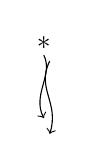
\begin{tikzpicture}[x=0.25cm,y=0.25cm]
\node at (0,4.6) {$*$};
\draw[->] (0,4) .. controls (0.5,3) and (-0.6,2) .. (0,0.8);
\draw[->] (0.3,3.7) .. controls (-0.4,2.3) and (0.8,1.6) .. (0.3,0);
\end{tikzpicture}}}
\diagram{\begin{tikzcd}[ampersand replacement=\&]
Y \& Y' \arrow[l,"g"'] \arrow[d,"i'"]\\
X \arrow[u,"\unsure{i}"] \& X' \arrow[l,"f"]
\end{tikzcd}}
\[
g^*(\mathbb{R}i^!)\longrightarrow(\mathbb{R}i'^!)f^*
\]
un isom. Tensorisant par
$T_{Y'/Y}$ et \unsure{shiftant} les degrés, il
revient au même de prouver que l'hom
naturel
\[
(\mathbb{R}^!g\deleted{\unsure{*}})(\mathbb{R}i^!)\longrightarrow(\mathbb{R}i'^!)(\mathbb{R}^!f)
\]
est un isom. Or \deleted{\unsure{par}} les th. de dualité
pour $f,g,i,i'$ nous disent essentiellement que
les deux mbs sont ``adjoints'' de
$(\mathbb{R}_!i)(\mathbb{R}_!g)$ et de $(\mathbb{R}_!f)(\mathbb{R}_!i')$, or ces derniers
sont canoniquement isomorphes. Il faut évidemment
prouver que l'\deleted{hom} isom \deleted{\unsure{ainsi}} précédent est bien
``adjoint'' de l'hom $(*)$, ce que je \unsure{suppose} fait.
Je vois un \unsure{ennui} de \unsure{degré|degrés}, car il faudrait
savoir, lorsqu'on prend un \unsure{complexe} $F\in\operatorname{Ob}\mathrm{C}(X)$,
\mspage{57}
